\documentclass{article}
\usepackage[utf8]{inputenc}

\usepackage{Mmbase}
\usepackage{tikz-imagelabels}
\usepackage{wrapfig}
\usetikzlibrary{animations}

\pagestyle{fancy}
\fancyhf{}

\fancyhead[C]{\rightmark}
\cfoot{\thepage}

\renewcommand{\sectionmark}[1]{%
  \markright{\textbf{\MakeUppercase{\thesection.\ #1}}}}%
  
%\titleformat{\subsection}[runin]
%{\normalfont\large\bfseries}{\thesubsection}{1em}{}

\titlelabel{\thetitle.\quad}

\renewcommand{\headrulewidth}{1pt}
\renewcommand{\footrulewidth}{1pt}

\date{ }


\definecolor{purple1}{RGB}{155,58,156}
\definecolor{yellow2}{RGB}{255,200,013}
\definecolor{blue3}{RGB}{0,155,230}
\definecolor{red4}{RGB}{236,013,021}
\definecolor{green5}{RGB}{016,171,061}

\definecolor{bubblegreen}{RGB}{103,184,104}
\definecolor{bubblegray}{RGB}{241,240,240}
\definecolor{midgray}{RGB}{94, 94, 94}
\definecolor{limegreen}{rgb}{0.2, 0.8, 0.2}


% \usepackage[many]{tcolorbox}
% \usepackage{xcolor}
% \usepackage{varwidth}
% \usepackage{environ}
% \usepackage{xparse}

% \newlength{\bubblesep}
% \newlength{\bubblewidth}
% \setlength{\bubblesep}{2pt}
% \AtBeginDocument{\setlength{\bubblewidth}{.75\textwidth}}

% \newcommand{\bubble}[4]{%
%   \tcbox[
%     on line,
%     arc=4.5mm,
%     colback=#1,
%     colframe=#1,
%     #2,
%   ]{\color{#3}\begin{varwidth}{\bubblewidth}#4\end{varwidth}}%
% }

% \ExplSyntaxOn
% \seq_new:N \l__ooker_bubbles_seq
% \tl_new:N \l__ooker_bubbles_first_tl
% \tl_new:N \l__ooker_bubbles_last_tl

% \NewEnviron{rightbubbles}
%  {
%   \begin{flushright}
%   \sffamily
%   \seq_set_split:NnV \l__ooker_bubbles_seq { \par } \BODY
%   \int_compare:nTF { \seq_count:N \l__ooker_bubbles_seq < 2 }
%   {
%     \bubble{bubblegreen}{rounded~corners}{white}{\BODY}\par
%   }
%   {
%     \seq_pop_left:NN \l__ooker_bubbles_seq \l__ooker_bubbles_first_tl
%     \seq_pop_right:NN \l__ooker_bubbles_seq \l__ooker_bubbles_last_tl
%     \bubble{bubblegreen}{sharp~corners=southeast}{white}{\l__ooker_bubbles_first_tl}
%     \par\nointerlineskip
%     \addvspace{\bubblesep}
%     \seq_map_inline:Nn \l__ooker_bubbles_seq
%      {
%       \bubble{bubblegreen}{sharp~corners=east}{white}{##1}
%       \par\nointerlineskip
%       \addvspace{\bubblesep}
%      }
%     \bubble{bubblegreen}{sharp~corners=northeast}{white}{\l__ooker_bubbles_last_tl}
%     \par
%   }
%   \end{flushright}
%  }
% \NewEnviron{leftbubbles}
%  {
%   \begin{flushleft}
%   \sffamily
%   \seq_set_split:NnV \l__ooker_bubbles_seq { \par } \BODY
%   \int_compare:nTF { \seq_count:N \l__ooker_bubbles_seq < 2 }
%   {
%     \bubble{bubblegray}{rounded~corners}{black}{\BODY}\par
%   }
%   {
%     \seq_pop_left:NN \l__ooker_bubbles_seq \l__ooker_bubbles_first_tl
%     \seq_pop_right:NN \l__ooker_bubbles_seq \l__ooker_bubbles_last_tl
%     \bubble{bubblegray}{sharp~corners=southwest}{black}{\l__ooker_bubbles_first_tl}
%     \par\nointerlineskip
%     \addvspace{\bubblesep}
%     \seq_map_inline:Nn \l__ooker_bubbles_seq
%      {
%       \bubble{bubblegray}{sharp~corners=west}{black}{##1}
%       \par\nointerlineskip
%       \addvspace{\bubblesep}
%      }
%     \bubble{bubblegray}{sharp~corners=northwest}{black}{\l__ooker_bubbles_last_tl}\par
%   }
%   \end{flushleft}
%  }
% \ExplSyntaxOff





\begin{document}




\begin{titlepage}

\begin{center}
    \vspace*{5cm}
    \huge IHM\\
    \text{ }\\
    \LARGE L2 Informatique\\
    \vfill
    \LARGE Groupe 7\\
    \LARGE WAHARTE Mathieu, ANDRIANTSEHENO Tanya,\\ HARTMANN Mathis\\
    \Large 2022-2023\\
\end{center}

\end{titlepage}

\newpage

%------------------------------------------------- TD1 -------------------------------------------------

\section{TD1 (21/10/2022)}

\subsection{VIM}
\quad VIM est un langage de commande puisque l'on peut clairement voir qu'il a une interface de type \textit{invite} et va réagir aux commandes de l'utilisateur (ici pour naviguer et éditer le document).
\text{ }\\
\text{ }\\
• Avantages :
\begin{itemize}
    \item[-] Le gain en vitesse est considérable lorsqu'on maîtrise complétement les commandes et spécificités de cette interface.
    \item[-] L'implémentation de de VIM est très peu gourmande en mémoire et en espace de stockage (comparé à d'autres éditeurs).
\end{itemize}
\text{ }\\
• Inconvénients :
\begin{itemize}
    \item[-] La courbe de progression de VIM est violente, de fait un utilisateur débutant aura beaucoup de difficultés à être efficace dans un premier temps.
    En effet, il y a un très grand nombre de commandes à maîtriser, ce qui le rends peu intuitif.
    \item[-] L'interface est peu élégante dû notamment à l'arrière plan foncé, contrastant avec les tons clairs des lettres, ce qui fatigue énormément l'oeil.
\end{itemize}

\hspace{5em}

\subsection{LibreOffice}
\quad LibreOffice utilise la manipulation directe ; en effet, son interface correspond au \textit{What You See Is What You Get} (on peut sélectionner du texte avec la souris, le mettre en gras en cliquant sur le bouton associé, sauvegarder le texte avec Cltr+S etc).
\text{ }\\
\text{ }\\
• Avantages :
\begin{itemize}
    \item[-] Plutôt intuitif : lorsque j'appuie sur les touches de mon clavier, les lettres correspondantes apparaissent directement sur l'interface.
    \item[-] L'interface est complète, on peut réaliser quasiment tout ce dont un utilisateur normal et même avancé pourrait souhaiter d'un éditeur de texte.
\end{itemize}
\text{ }\\
• Inconvénients :
\begin{itemize}
    \item[-] Du aux mises à jour itératives et additives, l'utilisateur peut se sentir noyé sous l'omniprésence d'options et fonctionnalités ; l'interface devient ainsi lourde.
\end{itemize}

\hspace{5em}

\subsection{iOS Notes}
\quad Notes utilise la manipulation directe puisque l'on réalise toutes les act


\text{ }\\
\text{ }\\
• Avantages :
\begin{itemize}
    \item[-] intuitif car l'interface minimaliste est attrayante.
\end{itemize}
\text{ }\\
• Inconvénients :
\begin{itemize}
    \item[-] peu d'informations dès l'ouverture du fichier, cela est bien dommage car on ne peut pas profiter pleinement des options existantes.
\end{itemize}


\newpage

%------------------------------------------------- TD2 -------------------------------------------------

\section{TD2 (18/11/2022)}


\subsection{Youtube}
\quad Les tâches élémentaires sur la recherche et les filtres sur Ebay sont :\newline

• Bureau :
\begin{figure}[H]
    \centering
    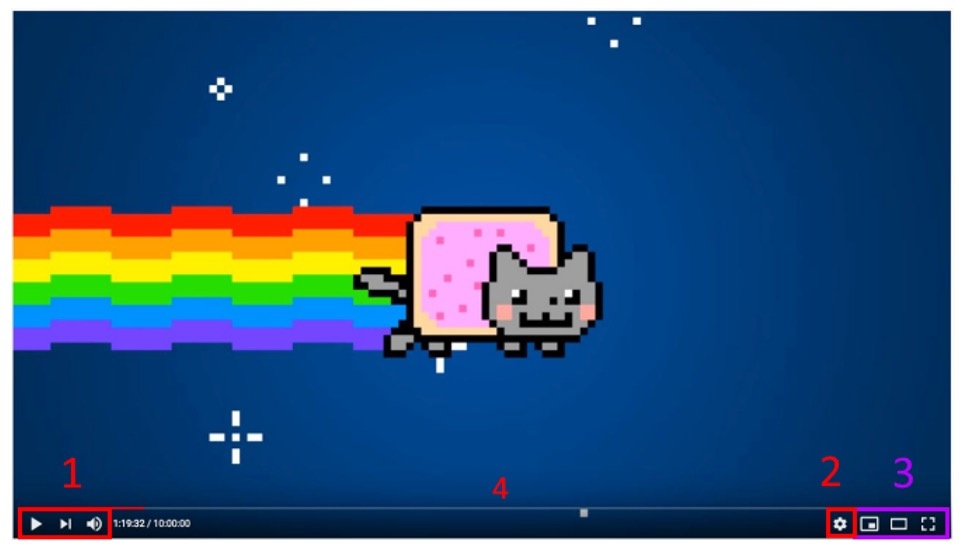
\includegraphics[width=0.8\linewidth]{Youtube_desktop.jpeg}
    \caption{Interface bureau de Youtube}
\end{figure}

\vspace{1cm}

\begin{enumerate}[label=\arabic*)]
    \item Tâche élémentaire : déclenchement d'actions. Action de bases : activation + pointage (bouttons en menu).
    \item  Tâche élémentaire : déclenchement d'actions. Action de bases : activation + pointage (menu pop-up).
    \item  élémentaire : déclenchement d'actions. Action de bases : activation + pointage (boutons en menu).
    \item Tâche élémentaire : transformation. Action de bases : activation + pointage (slider).
\end{enumerate}

\clearpage

\begin{figure}[H]
    \centering
    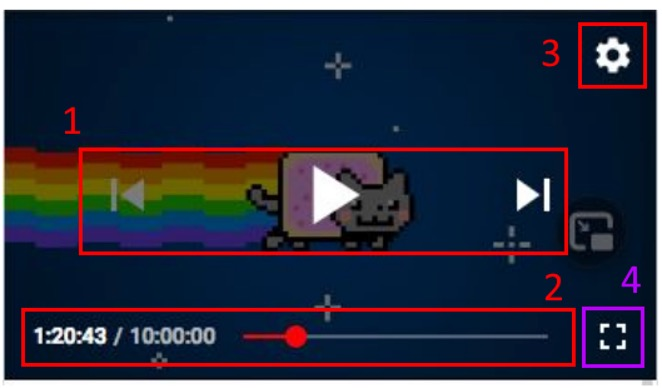
\includegraphics[width=0.8\linewidth]{Youtube_mobile.jpeg}
    \caption{Interface mobile de Youtube}
\end{figure}

\vspace{1cm}

\begin{enumerate}[label=\arabic*)]
    \item Tâche élémentaire : déclenchement d'actions. Action de bases : Tap (bouttons en "palette d'outils").
    \item  élémentaire : déclenchement d'actions/navigation (entrée de données ?). Action de bases : Tap et swipe (slider).
    \item  Tâche élémentaire : déclenchement d'actions. Action de bases : Tap (menu pop-up).
    \item  Tâche élémentaire : transformation. Action de bases : Tap (bouton).
\end{enumerate}

\vspace{2cm}

Dans les deux on retrouve des boutons accessible directement pour agir sur le flux vidéo (pause/play et skip) ainsi que d'autres pour modifier la taille de l'interface et accéder à des paramètres supplémentaires.\\
En revanche l'accès aux paramètres est plus compact sur télephone (l'espace y étant beaucoup plus limité); en contraste avec l'interface bureau où plusieurs raccourcis figurent pour rendre plus rapide ces actions.



\clearpage

\subsection{Ebay}
\quad Les tâches élémentaires sur la recherche et les filtres sur Ebay sont :\newline

• Bureau :
\begin{figure}[H]
    \centering
    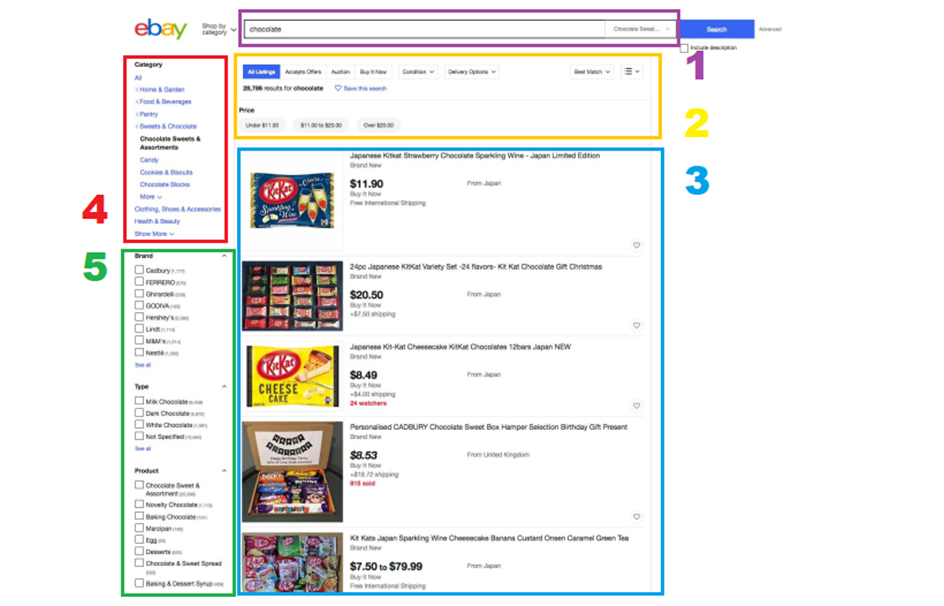
\includegraphics[trim=0cm 0cm 3cm 0cm,width=0.8\linewidth]{ebay_desktop.png}
    \caption{Interface bureau d'Ebay}
\end{figure}

\vspace{1cm}
\begin{enumerate}[label=\arabic*)]
    \item Tâche élémentaire : entrée de données. Actions de bases : entrée clavier (via clavier avec comme interacteur des boutons) et pointage (via curseur)
    \item Tâche élémentaire : déclenchement d'actions. Actions de bases : activation et pointage.
    \item Tâche élémentaire : choix de valeur. Actions de bases : activation et pointage.
    \item Tâche élémentaire : navigation. Actions de bases : activation et pointage.
    \item Tâche élémentaire : déclenchement d'actions. Actions de bases : activation et pointage.
\end{enumerate}
\clearpage


• Mobile :
\begin{figure}[H]
    \centering
    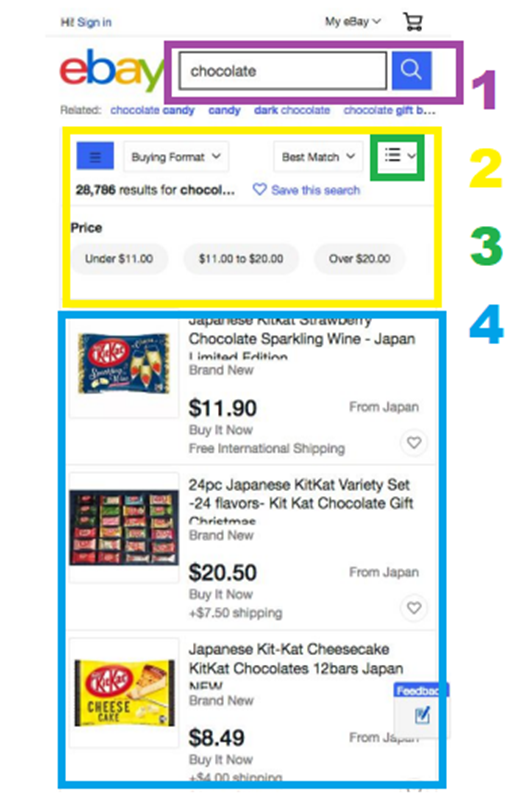
\includegraphics[width=0.4\linewidth]{ebay_mobile.png}
    \caption{Interface mobile d'Ebay}
\end{figure}

\vspace{1cm}
\begin{enumerate}[label=\arabic*)]
\item Tâche élémentaire : entrée de données. Actions de base : Tap (et Swipe)
\item Tâche élémentaire : déclenchement d’actions. Action de base : Tap
\item Tâche élémentaire : navigation et choix de valeur. Actions de base : Swipe et Tap
\item Tâche élémentaire : déclenchement d’actions. Actions de base : Tap
\end{enumerate}


\vspace{2cm}

Dans les deux versions, on peut dès qu’on arrive sur la page d’un résultat, parcourir les résultats (sur téléphone par un swipe et sur ordinateur via un curseur) et faire un choix parmi plusieurs propositions.\\
La principale différence est l’accès aux différents filtres (pour la version sur ordinateur c’est possible sur la même page tandis que pour la version mobile il faut au préalable cliquer sur un menu pour les différents filtres (numéro 3). C’est principalement par manque de place que les filtres ne sont pas présents sur la page directement. La barre de recherche est plus grande sur la version sur ordinateur que sur celle sur mobile par manque de place. 



\clearpage


\subsection{Draw.io}
\quad Les tâches élémentaires sur les formes sur le site draw.io sont :\newline

• Bureau :
\begin{figure}[H]
    \centering
\begin{tikzpicture}
    \node[anchor=south west,inner sep=0] at (0,0) {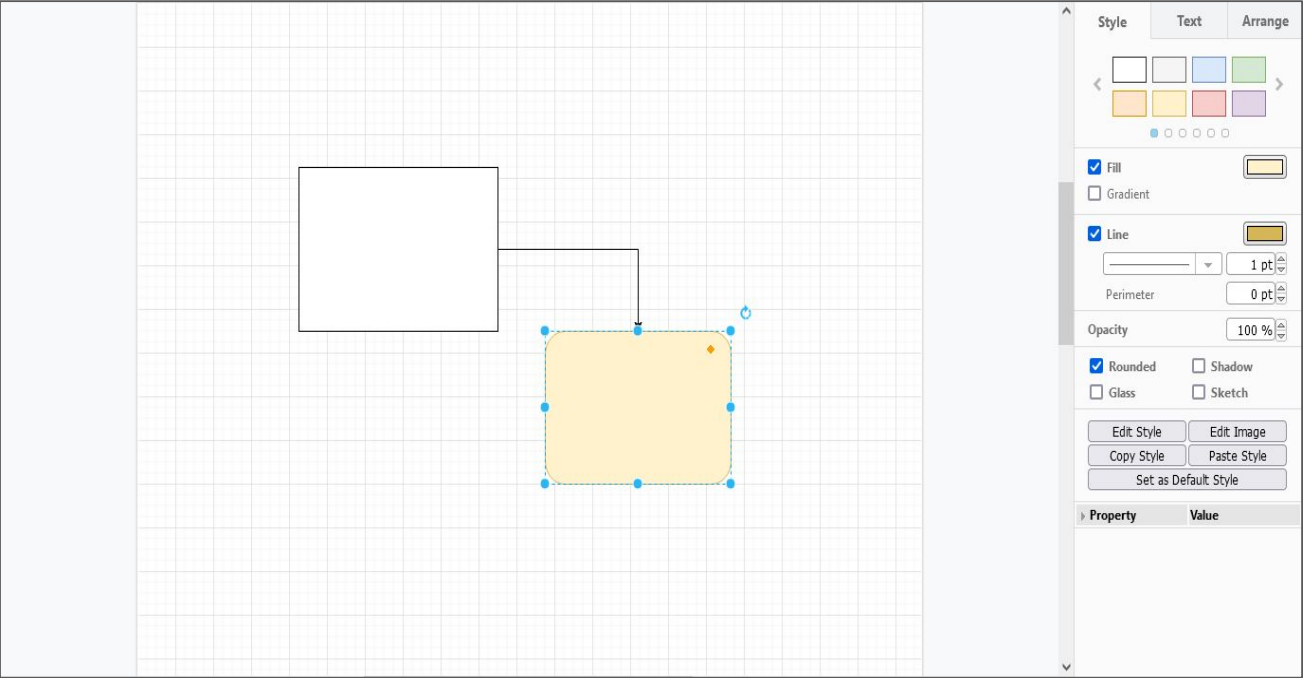
\includegraphics[width=0.8\textwidth]{drawio_desktop.png}};
    
    \draw[purple1,thick,rounded corners] (12.1,5.9) rectangle (14.3,7.01);
    \node[purple1, font=\large, right] at (14.4,6.86) {\textbf{1}};
    
    \draw[yellow2,thick,rounded corners] (11.95,5.2) rectangle (14.35,5.84);
    \node[yellow2, font=\large, right] at (14.44,5.74) {\textbf{2}};
    
    \draw[blue3,thick,rounded corners] (11.95,4.06) rectangle (14.35,5.12);
    \node[blue3,font=\large, right] at (14.44,5.02) {\textbf{3}};
    
    \draw[red4,thick,rounded corners] (11.95,2.97) rectangle (14.35,4.01);
    \node[red4, right, font=\large] at (14.44,3.91) {\textbf{4}};
    
    \draw[green5,thick,rounded corners] (7.92,3.73) rectangle (8.42,4.2);
    \node[green5,font=\large, right] at (8.42,4.15) {\textbf{5}};
    
    \draw[brown,thick,rounded corners] (11.977,7.08) rectangle (14.375,7.46);
    \node[brown, font=\large, right] at (14.44,7.35) {\textbf{6}};
\end{tikzpicture}

\caption{Interface bureau de Draw.io}
\end{figure}

\vspace{1cm}

\begin{enumerate}[label=\arabic*)]
    \item Tâche élémentaire : transformation/choix d'élément dans un ensemble. Action de base : activation et pointage (curseur).
    \item Tâche élémentaire : déclenchement d'actions. Action de base : activation et pointage (curseur).
    \item Tâche élémentaire : déclenchement d'actions et entrée de données. Action de base : activation + pointage, entrée clavier et activation + pointage (resp. curseur, compteur+combo box, curseur).
    \item Tâche élémentaire : entrée de données et déclenchement d'actions. Action de base : entrée clavier et activation + pointage (resp. compteur et cases à cocher + curseur).
    \item Tâche élémentaire : transformation. Action de base : tracé et activation (manipulation de poignées et rotation par clic du cercle).
    \item Tâche élémentaire : navigation. Action de base : activation et pointage (barre de menus).
\end{enumerate}
\clearpage


• Mobile :
\begin{figure}[H]
    \centering
    
\begin{tikzpicture}
    \node[anchor=south west,inner sep=0] at (0,0) {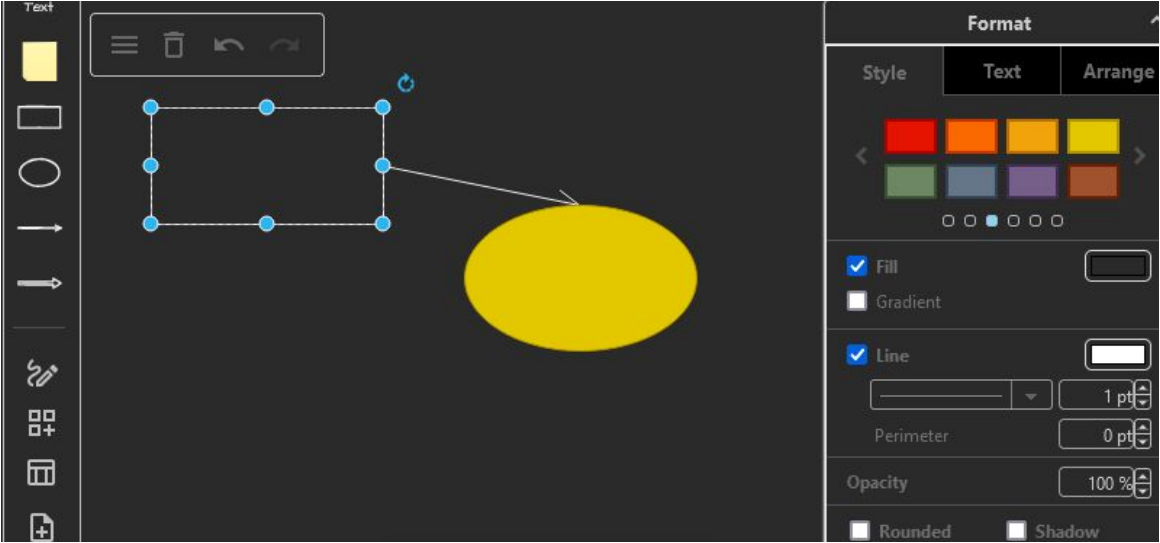
\includegraphics[width=0.8\textwidth]{drawio_mobile.png}};
    
    \draw[purple1,thick,rounded corners] (10.5,3.82) rectangle (14.3,5.4);
    \node[purple1,font =\large, right] at (14.44,5.2) {\textbf{1}};
    
    \draw[yellow2,thick,rounded corners] (10.35,2.8) rectangle (14.4,3.74);
    \node[yellow2, font=\large, right] at (14.44,3.59) {\textbf{2}};
    
    \draw[blue3,thick,rounded corners] (10.35,0.5) rectangle (14.4,2.7);
    \node[blue3, font=\large,right] at (14.44,2.5) {\textbf{3}};
    
    \draw[red4,thick,rounded corners] (4.52,5.2) rectangle (5.43,6.08);
    \node[red4, font=\large,right] at (5.5,5.89) {\textbf{4}};
    
    \draw[green5,thick,rounded corners] (1.1,5.75) rectangle (4.12,6.67);
    \node[green5, font=\large,right] at (4.14,6.4) {\textbf{5}};
    
    \draw[brown,thick,rounded corners] (10.5,5.54) rectangle (14.4,6.2);
    \node[brown,font=\large, right] at (14.44,6) {\textbf{6}};
    
    \draw[pink,thick,rounded corners] (0.06,0.05) rectangle (1.06,6.73);
    \node[pink, font=\large,right] at (1.12,0.3) {\textbf{7}};
\end{tikzpicture}

\caption{Interface mobile de Draw.io}
\end{figure}

\vspace{1cm}

\begin{enumerate}[label=\arabic*)]
    \item Tâche élémentaire : transformation/choix d'élément dans un ensemble. Action de base : Tap.
    \item Tâche élémentaire : déclenchement d'actions. Action de base : Tap.
    \item Tâche élémentaire : déclenchement d'actions et entrée de données. Action de base : Tap, entrée clavier (compteur+combo box), Tap et Tap.
    \item Tâche élémentaire : transformation. Action de base : hold \& drag (manipulation de poignées) et Tap (cercle).
    \item Tâche élémentaire : déclenchement d'actions. Action de base : Tap (palette d'outils).
    \item Tâche élémentaire : navigation. Action de base : Tap (barre de menus).
    \item Tâche élémentaire : déclenchement d'actions. Action de base : Tap (palette d'outils).
    
\end{enumerate}

\vspace{2cm}

Dans les deux version on peut sélectionner un style prédéfini ou le customiser à l'aide de compteurs, de checkboxes et de menus pop-up pour les couleurs. De plus, il est aussi possible dans les deux cas de redimensionner la forme via les poignées ou la faire tourner via le cercle et d'accèder à d'autre menus.
En revanche, ils se distingue de par une grille sur la version bureau (pratique pour l'alignement mais réduit la lisibilité sur mobile), un menu sur le côté avec des actions rapides sur mobile (pour éviter trop de navigation des menus, ce qui est dur sur mobile) et un menu d'outils rapides pour les mêmes raisons (et car les raccourcis Cltr+Z et Suppr ne sont pas disponible sur mobile).



%\newpage
% common :\\
% quick styles select $\ra$ click to select menu with multiple panels\\
% fill/gradient mode $\ra$ checkbox + fill color in pop-up color select panel\\
% type/color/strength of line $\ra$ resp. dropdown+counter, pop-up panel, counter\\
% opacity $\ra$ percentage counter\\
% transform size and shape of obj $\ra$ blue circles and rotate via arrow\\
% tabs for text and arrange\\
% \text{ }\newline


% on desktop :\\
% edit/copy\&paste style + set as default $\ra$ buttons $|$ power user actions ; not indispensable and takes precious space on a small screen\\
% grid $|$ help align items ; would reduce readability on mobile\\
% \text{ }\newline


% on mobile :\\
% undo, delete and align $\ra$ moving panel with buttons $|$ to avoid mobile users to navigate too much in menus which is hard on mobile and not so much on desktop\\
% quick actions (text, arrows, circle, rectangle) + document actions $\ra$ side menu $|$ same reasoning\\

% \newpage

% \begin{annotationimage}{width=6cm}{drawio_mobile.png}
% \draw[annotation left = {Atlas at 0.3}] to (0.11,0.4);
% \draw[annotation left = {Pleione at 0.55}] to (0.11,0.49);
% \draw[annotation left = {Alcyone at 0.8}] to (0.39,0.45);
% \draw[annotation below = {Merope at 0.5}] to (0.58,0.28);
% \draw[annotation right = {Electra at 0.3}] to (0.84,0.45);
% \draw[annotation right = {Caleano at 0.75}] to (0.85,0.64);
% \draw[annotation above = {Maia at 0.4}] to (0.67,0.72);
% \draw[annotation above = {Taygeta at 0.9}] to (0.78,0.82);
% \draw[image label = {M45 at south east}];
% \end{annotationimage}


\newpage

%------------------------------------------------- TD3 -------------------------------------------------

\section{TD3 (25/11/2022)}

\begin{figure}[H]
\centering
\begin{tikzpicture}
    \filldraw[fill=lightgray] (0,0) rectangle (15,10);
    
    %------ play button -------
    \filldraw[fill=red] (7.5,1) circle [radius=0.4];
    \filldraw[fill=white] (7.43,1.2) -- (7.43,0.8) -- (7.66,1) -- cycle;
    
    %------ truc de gauche -----
    \filldraw[fill=white] (0.7,1.7) rectangle (5,9.3);
    \node[right,align=center] at (1.5,8.5){$\text{Y}^2+\text{X}^2$-MEN\\ APOCALYPSE};
    \node[right] (film) at (0.7,7.2) {
\includegraphics[width=4.05cm]{film.jpeg}};
    \node[right,align=left] at (0.7,5.6){\footnotesize Lorem ipsum dolor sit amet,\\\footnotesize consectetur adipiscing elit.\\\footnotesize Mauris non ante rutrum.};
    \node[right] (fav) at (1.6,3.3) {
\includegraphics[width=0.5cm]{fav.png}};
    \node[right] at (1.58,2.83){\scriptsize vote};
    \node[right] (watched) at (2.9,3.3) {
\includegraphics[width=0.5cm]{watched.png}};
    \node[right] at (2.68,2.83){\scriptsize regardé};
    
    %------ truc du milieu ------
    \filldraw[fill=white] (5.6,7) rectangle (9.4,4);
    \node[right] at (5.72, 6.1){Termination 3}; \node[right, orange] at (8.73, 6.1){1};
    \node[right] at (5.72, 5.5){Titanium}; \node[right, limegreen] at (8.64, 5.5){32};
    \node[right] at (5.72, 4.9){Interaction}; \node[right, red] at (8.73, 4.9){0};
    
    %------ truc de droite ----
    \filldraw[fill=white] (10,1.7) rectangle (14.3,9.3);
    \path [fill=darkgray] (10,9.3) rectangle node[white,align=center]{User \#24987 \\ \scriptsize Online 5min ago} (14.3,8);
    \path [rounded corners=5pt, fill=bubblegray] (10.12, 5.43) rectangle (12.6, 6.43);  \node[black,right,align=left,text width=4cm] at (10.16,5.9){Thorus 2 \\was amazing !};
    \path [rounded corners=5pt, fill=bubblegreen] (12.45, 4.69) rectangle (14.2, 5.39);  \node[white,left] at (14.05,5.04){I agree !};
    \path [rounded corners=5pt, fill=bubblegray] (10.12, 3.35) rectangle (11.92, 4.74);  \node[black,right,align=left,text width=4cm] at (10.16,4.03){we should \\hang-out\\ sometime};
    \path [rounded corners=5pt, fill=bubblegreen] (12, 2.7) rectangle (14.2, 3.4);  \node[white,left] at (14.05,3.05){movie tn ?};
    \path [rounded corners=7pt,fill=midgray] (10, 1.71) rectangle node[white]{\small Text message} (14.3, 2.3);
    %\node at (12,3) {\bubble{bubblegreen}{rounded~corners}{white}{This film was amazing}};
    
\end{tikzpicture}
\caption{Croquis interface Newtflix}
\label{fig:croquis}
\end{figure}



% \begin{rightbubbles}
% Left-aligned gray bubbles (241, 240, 240) with black text

% Right-aligned green bubbles (103, 184,104) with white text

% Bubbles only break after a paragraph (equivalent to an enter press 
% when chatting). Long message with multiple lines will be kept in one bubble.

% Left and right edges are round.
% \end{rightbubbles}

% \begin{leftbubbles}
% Left-aligned gray bubbles (241, 240, 240) with black text

% Right-aligned green bubbles (103, 184,104) with white text

% Bubbles only break after a paragraph (equivalent to an enter press 
% when chatting). Long message with multiple lines will be kept in one bubble.

% Left and right edges are round.
% \end{leftbubbles}

% \begin{rightbubbles}
% Single
% \end{rightbubbles}

% \begin{leftbubbles}
% End
% \end{leftbubbles}

\end{document}
